%==============================================================================
%  Three Mechanisms Inflate Reported Performance on a Widely Used Public
%  Chronic Kidney Disease Benchmark
%
%  IEEE conference format (IEEEtran). To build:
%      pdflatex ieee_paper && pdflatex ieee_paper
%  (run twice so cross-references resolve).
%
%  For the journal format instead, change the class options on the next
%  line to [journal]{IEEEtran} and remove \IEEEpeerreviewmaketitle.
%
%  Every numerical value in this paper is taken from a generated table in
%  reports/tables/ of the accompanying repository. The comment above each
%  table names its source file.
%==============================================================================
\documentclass[conference]{IEEEtran}

\usepackage{cite}
\usepackage{amsmath,amssymb}
\usepackage{graphicx}
\usepackage{booktabs}
\usepackage{multirow}
\usepackage{xcolor}
\usepackage{url}
\usepackage[hidelinks]{hyperref}

\graphicspath{{figures/}}

% Compact, consistent table type.
\newcommand{\tabhead}[1]{\textbf{#1}}
\renewcommand{\arraystretch}{1.15}

\begin{document}

\title{Three Mechanisms Inflate Reported Performance\\
on a Widely Used Public Chronic Kidney Disease Benchmark}

%------------------------------------------------------------------------------
% TODO(author): replace the placeholder block below before submission.
% Left unfilled deliberately rather than guessed.
%------------------------------------------------------------------------------
\author{\IEEEauthorblockN{Author Name}
\IEEEauthorblockA{\textit{Department} \\
\textit{Institution}\\
City, Country \\
email@institution.edu}
}

\maketitle

%==============================================================================
\begin{abstract}
Machine-learning studies on the public UCI chronic kidney disease (CKD)
benchmarks routinely report accuracy at or near 100\%. We ask what produces
those numbers. Under repeated nested cross-validation with programmatically
enforced leakage control, we identify and quantify three distinct mechanisms,
none of which is predictive ability. First, \emph{target leakage}: the
released file contains an exact copy of the outcome, a post-diagnosis stage
label, and the diagnostic eGFR value; including them takes every feature
configuration to ROC-AUC 1.000. Second, and larger, \emph{case-mix
composition}: with every prohibited column removed, models still separate all
200 patients out of fold, because 84\% of cases carry stage 3--5 disease and
haemoglobin alone reaches univariate ROC-AUC 0.968; in an exploratory, post
hoc and statistically underpowered subgroup of the 21 early-stage cases,
sensitivity falls from 0.969 to 0.905, a hypothesis-generating signal
requiring confirmation in a larger prospectively defined cohort. Third, and
least visible,
\emph{pseudo-external validation}: a record-level provenance check shows that
the 2015 and 2020 UCI releases, treated in the literature as independent
cohorts, share their patients. All 200 patients of the 2020 release match
into the 2015 release (maximum bipartite match fraction 1.000 against a
permutation null of $0.003 \pm 0.003$), 187 of them uniquely, with zero
contradictions across ten categorical variables that took no part in the
matching. Of 13 surveyed studies, three validate across these releases as
though independent and one merges them into a single training set.
Recovering the original measurements further shows that the published
discretisation destroys 0.266 ROC-AUC of univariate signal in serum
creatinine while changing no multivariable conclusion, and that 339 missing
cells were silently filled with constants whose absence is strongly
outcome-associated. Finally, as a \emph{transportability probe} rather than a
definitive external validation, we transfer the models unchanged to an
independent critical-care cohort---the only registered source carrying the
same measurements on different patients---where discrimination falls from
0.997 to 0.70 (95\% CI 0.59--0.80) and Brier rises from 0.014 to 0.42. With
20 cases in a markedly different clinical setting, this difference cannot be
attributed to internal optimism alone: small-sample uncertainty, case mix,
feature definition, missingness and genuine distribution shift all plausibly
contribute. We release the full pipeline, including a reusable provenance
gate that blocks non-independent cohorts from supporting external claims, and
a diagnostic protocol that would have flagged this benchmark before any model
was fitted.
\end{abstract}

\begin{IEEEkeywords}
chronic kidney disease, data leakage, spectrum bias, transportability,
external validation, benchmark quality, clinical prediction models,
reproducibility
\end{IEEEkeywords}

%==============================================================================
\section{Introduction}

Chronic kidney disease affects roughly 9\% of the world's population and
caused an estimated 1.2 million deaths in 2017, with the burden falling
disproportionately on regions where diagnostic laboratory capacity is
limited~\cite{gbd2020}. CKD is defined by abnormalities of kidney structure or
function persisting beyond three months, operationalised principally through
estimated glomerular filtration rate (eGFR) and albuminuria~\cite{kdigo2024}.
Because early CKD is largely asymptomatic, detection depends on testing rather
than presentation.

That clinical importance is why the public UCI CKD datasets have become
standard benchmarks: they are small, tidy, and answer a question that matters.
It is also why results reported on them deserve scrutiny. \emph{A benchmark on
which almost every method reports near-perfect accuracy has stopped
discriminating between methods}, and the interesting question becomes what, in
the data, produces the ceiling.

A targeted illustrative review of 13 studies using this dataset or its parent
release (Section~\ref{sec:priorwork}) shows that such results exist in the
published record: of the three studies we could verify from the source text,
two report headline accuracy at or above 99\%, and one reports 99.5\% after
merging the two releases into a single training set. The review is not
systematic and supports no claim about how common these practices are. Its
purpose here is to establish that the failure modes we go on to characterise
are not hypothetical.

This paper began as an ordinary applied study of whether inexpensive
variables---history, examination, a urine dipstick---could predict CKD status.
It was built with leakage control enforced in code and repeated nested
cross-validation. That construction produced an uncomfortable result: every
valid configuration sat at the discrimination ceiling, with no prohibited
column involved. An automated tripwire (``perfect performance means a bug'')
fired, and the investigation into why became the study.

\subsection{Contributions}

\begin{enumerate}
  \item We identify and separately quantify \textbf{three mechanisms} that
        drive measured performance on this benchmark toward 1.0, and show that
        the largest is not the one the literature discusses.
  \item We provide \textbf{record-level evidence} that two UCI releases treated
        as independent cohorts share their patients, invalidating published
        cross-dataset validations between them, and release the provenance
        check as reusable, dataset-agnostic machinery.
  \item We \textbf{recover the original continuous measurements} for the
        analysed cohort, making the cost of the published discretisation
        measurable \emph{within-cohort}, and in doing so surface undocumented
        constant imputation in the released file.
  \item We report an \textbf{honest uncertainty interval} obtained by
        bootstrapping the entire nested procedure, which is 1.7--2.7$\times$
        wider than the conventional prediction-level interval.
  \item We report a \textbf{transportability probe} on the one independent
        source carrying the same measurements, in which discrimination near
        1.0 falls to 0.70 on patients the models never saw. With 20 cases in
        a different clinical setting it is a stress test rather than a
        definitive external validation, and we are explicit about the several
        mechanisms that could produce the difference.
  \item We propose a \textbf{diagnostic protocol} for deciding whether a
        benchmark can distinguish methods at all, and report a negative
        result about one of its own components.
\end{enumerate}

%==============================================================================
\section{Related Work: A Targeted Illustrative Review}
\label{sec:priorwork}

Recent surveys of machine learning for CKD~\cite{kabir2026} note that the
majority of studies rely on the UCI-2015 release~\cite{uci2015}, and that many
include serum creatinine or eGFR as inputs---a practice Kabir \emph{et al.}
describe as introducing ``information leakage and circular reasoning,'' since
those biomarkers are themselves the clinical criteria defining the outcome.

\textbf{This section is a targeted illustrative review, not a systematic
one.} We state that plainly because the distinction bounds every claim we
make about the literature. Studies were identified from the reference list of
one recent survey~\cite{kabir2026} and from citation trails of the two
dataset releases; there was no protocol-driven multi-database search, no
independent double screening, and no attempt at exhaustive coverage. The
sample is therefore sufficient to demonstrate that particular practices
\emph{occur}, and insufficient to estimate how often they occur. We make no
prevalence claim about the literature anywhere in this paper.

Of the 13 studies examined, three could be verified from full text or
abstract; the remaining ten sit behind paywalls we could not access, and
their coding is \emph{attributed} to the published comparison table
of~\cite{kabir2026} rather than independently confirmed. Consistent with the
above, \textbf{the ten unverified studies support no quantitative statement
in this paper}: every count we report is either over all 13 studies as a
description
of the sample we assembled, or restricted to the three verified studies, and
Table~\ref{tab:lit} labels which is which.

Among the verified studies, Islam \emph{et al.}~\cite{islam2023} report 99.16\%
accuracy on the 2015 release with serum creatinine among the predictors and no
external validation, and Hossain \emph{et al.}~\cite{hossain2025} report 99.5\%
accuracy after \emph{merging} the two releases into a single training set,
with reported accuracies reaching 100\% in cross-release validation. Both
figures are consistent with the mechanisms identified below; the second is
directly affected by the cohort-overlap finding of
Section~\ref{sec:mech3}.

% Source: reports/tables/table_26_prior_work_summary.csv
\begin{table}[t]
\caption{Targeted illustrative review ($N=13$ studies examined). Rows marked
\emph{attributed} rest on a published comparison table~\cite{kabir2026}, not
on our own reading, and support no quantitative claim. This is not a
systematic sample; no prevalence should be inferred from it.}
\label{tab:lit}
\centering
\footnotesize
\setlength{\tabcolsep}{3.5pt}
\begin{tabular}{lrl}
\toprule
\tabhead{Quantity} & \tabhead{Value} & \tabhead{Basis} \\
\midrule
Studies examined & 13 & our sample \\
Independently verified & 3 & full text / abstract \\
Not accessible (paywalled) & 10 & --- \\
Verified headline metrics $\geq 0.99$ & 2 of 3 & verified only \\
Coded as using creatinine or eGFR & 9 & attributed \\
Using the 2020 release or a merge & 4 & attributed \\
Cross-validating between the releases & 3 & attributed \\
With a genuinely external cohort & 1 & verified \\
\bottomrule
\end{tabular}
\end{table}

The purpose of the table is existence, not prevalence: it establishes that
studies reporting near-ceiling accuracy on this benchmark, studies using
creatinine or eGFR as inputs, and studies validating across the two releases
all exist in the published record --- the last of which
Section~\ref{sec:mech3} shows to be invalid. How common each practice is
would require the systematic review this section is not.

%==============================================================================
\section{Intended Use, Data, and Provenance}
\label{sec:data}

\subsection{Intended use, and why this dataset cannot fix one}
\label{sec:intendeduse}

A prediction model is interpretable only against a stated intended use.
Table~\ref{tab:intendeduse} sets out the use this benchmark is usually taken
to support, and what the released file actually permits.

% Source: authors' specification; no computed values.
\begin{table}[t]
\caption{Intended-use specification. The right column records what the
released data can support, which is in several places less than the
benchmark's common framing assumes.}
\label{tab:intendeduse}
\centering
\footnotesize
\setlength{\tabcolsep}{3pt}
\begin{tabular}{p{2.35cm}p{5.5cm}}
\toprule
\tabhead{Element} & \tabhead{Specification / what the data permit} \\
\midrule
Population & Adults assessed for suspected kidney disease. The release
documents no eligibility criteria, recruitment window or consecutive
sampling, so the population is not reconstructible. \\
Setting & Hospital-based, single centre. Not a community or primary-care
series. \\
Index time & \emph{Not identifiable.} No timestamps exist; the file gives no
ordering between examination, dipstick, venepuncture and diagnosis. \\
Information at index & Cannot be established per patient, for the same
reason. Availability is therefore assigned per \emph{variable} by clinical
reasoning (Table~\ref{tab:leakage}), not observed. \\
Outcome & \texttt{class} $\in$ \{ckd, notckd\}, as labelled. Chronicity ---
required by the KDIGO definition~\cite{kdigo2024} --- cannot be verified
from a single cross-sectional record. \\
Task type & \emph{Ambiguous.} Because index time is unidentifiable and
diagnostic measurements are contemporaneous with labelling, the task is
better described as retrospective case--control discrimination than as
screening, diagnosis or prognosis. \\
Decision supported & None established. No referral, treatment or triage
decision can be attached to a prediction whose index time is unknown. \\
\bottomrule
\end{tabular}
\end{table}

Three of those rows are blank in a way that matters. Without an index time,
``available at prediction time'' cannot be verified per patient; without
chronicity, the outcome is not the KDIGO construct; and without a defined
decision, calibration and thresholds have no operating context. We therefore
do not treat this work as a prediction-model development study, and no result
in it should be read as one.

\textbf{This paper is a methodological benchmark audit.} Its object is the
measurement process: what properties of the released data explain the
performance reported on it, and what checks would have revealed those
properties in advance. Where models are fitted, they are instruments for
probing the data, not candidate clinical tools.

\subsection{The analysed release}

We analyse \texttt{ckd-dataset-v2.csv}, 200 patient records in 29 columns,
distributed by the UCI Machine Learning Repository as \emph{Risk Factor
Prediction of Chronic Kidney Disease}~\cite{uci2023}. The outcome
\texttt{class} is 128 CKD (64.0\%) and 72 non-CKD. Two rows immediately
following the header are metadata, not observations, and are removed in a
single place in the codebase.

With 72 minority events and 25 candidate predictors in the full valid
configuration, the dataset provides 2.88 events per predictor---far below
accepted minimums for prediction-model development~\cite{riley2019}. The study
is therefore underpowered for model development by construction and is
presented as a measurement exercise on the benchmark itself.

\subsection{Two properties that shape everything}

\textbf{The data are pre-discretised.} Every continuous variable was binned
into interval strings before release (\texttt{sg} as
\texttt{1.019 - 1.021}, \texttt{bgr} as \texttt{< 112}). We encode each label
by a single representative value---the midpoint of a closed bin, the finite
edge of an open one. This mapping is a pure function of one cell's text: it
uses no cross-row statistics and no outcome information, so it cannot transfer
information between folds, which is why it may legitimately be applied before
splitting.

\textbf{The documented provenance is contradicted by the data.} The release
documents collection at a named hospital in Bangladesh. Section~\ref{sec:mech3}
shows that all 200 of these patients appear in the 2015 UCI
release~\cite{uci2015}, documented as an Indian hospital. We report the
measurement and take no view on how the discrepancy arose; readers should
treat the stated site, country and year as unverified. No claim in this paper
rests on them.

\subsection{Feature-availability and leakage taxonomy}
\label{sec:taxonomy}

Because index time is unidentifiable per patient
(Section~\ref{sec:intendeduse}), availability is assigned per variable and
recorded declaratively. \texttt{data/feature\_registry.csv} holds, for each
of the 29 columns, its leakage category, availability at the proposed index
time, whether it participates in constructing or staging the outcome, its
cost tier, the configurations it may enter, the evidence for the
classification, and an uncertainty flag. The feature configurations used in
every experiment are \emph{derived} from that registry rather than
maintained beside it, and a test asserts the derivation reproduces the
declared configurations exactly, so a classification cannot drift from the
configuration depending on it.

The taxonomy separates categories that are often conflated
(Table~\ref{tab:leakage}). Two are barred outright. Two more are admissible
but carry interpretation caveats that the manuscript discloses wherever they
matter: \emph{incorporation risk}, where a legitimate contemporaneous
measurement is also an input to the diagnostic criterion, and
\emph{consequence of advanced disease}, where a variable is real and
measurable but derives its discriminative value from severity rather than
from early detectability.

% Generated by scripts/24_make_latex_tables.py -- do not edit.
\begin{table}[t]
\caption{Feature-availability and leakage taxonomy. Categories are assigned in \texttt{data/feature\_registry.csv}, from which the feature configurations are derived; a test asserts the two agree. Prohibited categories cannot enter any clinically valid configuration.}
\label{tab:leakage}
\centering
\footnotesize
\setlength{\tabcolsep}{3pt}
\begin{tabular}{p{2.05cm}p{3.05cm}p{2.35cm}}
\toprule
\tabhead{Category} & \tabhead{Variables} & \tabhead{Decision} \\
\midrule
Direct outcome copy & \texttt{affected}, \texttt{class} & \textbf{Excluded} from every valid configuration \\
Deterministic derivative & \texttt{grf}, \texttt{stage} & \textbf{Excluded} from every valid configuration \\
Incorporation risk & \texttt{bu}, \texttt{sc} & Retained; incorporation risk disclosed \\
Consequence of advanced disease & \texttt{ane}, \texttt{hemo}, \texttt{pcv}, \texttt{rbcc} & Retained; severity-driven signal disclosed \\
Uncertain provenance & \texttt{appet}, \texttt{bp (Diastolic)}, \texttt{bp limit}, \texttt{cad}, \texttt{dm}, \texttt{pot}, \texttt{rbc}, \texttt{su} & Retained where tiering is conservative \\
Legitimate pre-index & \texttt{age}, \texttt{al}, \texttt{ba}, \texttt{bgr}, \texttt{htn}, \texttt{pc}, \texttt{pcc}, \texttt{pe}, \texttt{sg}, \texttt{sod}, \texttt{wbcc} & Retained \\
\bottomrule
\end{tabular}
\end{table}


\subsection{Prohibited columns}

Three columns cannot be legitimate predictors. \texttt{affected} is an exact
one-to-one copy of the outcome (Cram\'er's $V = 1.0$ across all 200 rows).
\texttt{stage} is a post-diagnosis staging label, 100\% CKD at stages s3 and
s5. \texttt{grf} is the eGFR value from which staging is banded and by which
CKD is defined. A model given these is performing lookup, not prediction: at
the moment of assessment none of the three exists yet.

%==============================================================================
\section{Methods}

\subsection{Feature configurations}

Six configurations are compared. \texttt{leaky\_model} (28 variables) is
\emph{deliberately invalid}: it adds the three prohibited columns and exists
solely to quantify their effect. It is labelled INVALID in every table and
figure and is never quoted outside the leakage audit. The valid
configurations are \texttt{full\_valid} (25), \texttt{laboratory} (14),
\texttt{low\_cost} (11: history, examination, urine dipstick),
\texttt{clinical\_only} (8), and \texttt{low\_cost\_plus\_urine\_micro} (15).
Machine-checked invariants hold: \texttt{clinical\_only} $\subset$
\texttt{low\_cost} $\subset$ \texttt{full\_valid}, and
\texttt{low\_cost} $\cup$ \texttt{laboratory} $=$ \texttt{full\_valid}.

The dataset ships no data dictionary. Ten variables whose meaning could not be
settled from the file are flagged \texttt{uncertain} rather than given
invented interpretations. The most consequential is \texttt{ane} (anaemia),
which could be recorded clinically at no cost or read from a blood count;
because its provenance is unresolved it is excluded from the low-cost
configuration. This is the conservative choice: it can only \emph{understate}
low-cost performance.

\subsection{Leakage prevention, enforced in code}
\label{sec:leakageprev}

Prevention operates in three independent layers. \emph{Declaration}: a single
module names every prohibited column and each configuration's exact contents.
\emph{Runtime guard}: every pipeline begins with a guard that raises at
\texttt{fit} \textbf{and} at \texttt{transform}, so a prohibited column
smuggled in at prediction time also fails; it \emph{raises rather than drops},
because silently dropping would conceal a caller's bug. \emph{Assertion}: a
cleanliness check runs over every pipeline before any work is done. The key
adversarial test hands a valid pipeline the \emph{entire} dataframe, including
all prohibited columns, and requires it to refuse rather than quietly select
its own subset.

\subsection{Validation design}

\textbf{The effective sample is 200 unique patients.} Models are evaluated
under 5-fold outer, 4-fold inner nested stratified cross-validation repeated
5 times. This yields 25 outer test folds, but these are five repartitions of
the same 200 patients: each patient is evaluated exactly once per repeat, so
the design produces \emph{5 out-of-fold evaluations per patient}, not 25
independent test sets. Repeated evaluations of the same individuals do not
increase the effective sample size, and no interval reported here treats them
as though they did. Per-patient probabilities are averaged across repeats
before any metric is computed, so each patient contributes one value; the
repeats reduce partition noise, not sampling uncertainty. Across the full
grid of configurations, models and calibration methods the pipeline stores
108{,}000 prediction rows, which are repeated evaluations of these 200
patients and are reported only as an artefact size.

The nested design is used because selecting hyper-parameters and estimating
performance on the same folds is a known source of optimism~\cite{varma2006}. Six model families are compared: a
prevalence dummy, penalised logistic regression, random forest, RBF support
vector machine, XGBoost, and an explainable boosting machine
(EBM)~\cite{nori2019} configured as a pure additive model. Imputation, scaling, hyper-parameter selection,
calibration and threshold selection all occur strictly within training folds.
Uncalibrated, Platt and isotonic probabilities are compared. Confidence
intervals come from a stratified patient-level bootstrap (2000 resamples);
Section~\ref{sec:honest} replaces these with an interval for the whole
procedure.

Calibration slope and intercept follow the standard logistic recalibration
framework~\cite{vancalster2016}. Two design details are worth stating because
they change reported numbers. Calibration statistics are computed
\emph{within} each repeat and then summarised: averaging a patient's
probability across repeats shrinks it toward the centre and biases the slope
upward. And complete separation is
\emph{detected} rather than optimised through---under separation the logistic
recalibration slope has no maximum-likelihood solution, and an optimiser still
returns a number (values in the hundreds were observed before the check was
added), so such slopes are reported as undefined.

\subsection{The provenance gate}
\label{sec:gate}

Before any dataset may support an external claim, it passes a record-level
check. Each patient in the analysed file is a vector of intervals over 13
shared variables. A candidate record is \emph{compatible} with a patient if
the outcome matches and every shared value falls inside the corresponding
interval; missing values are treated as compatible, which can only
\emph{raise} the match fraction and is therefore the conservative direction
for a gate. We compute the maximum bipartite matching between patients and
candidate records under this relation, and calibrate the observed matching
against permutations that shuffle each candidate column independently,
preserving every marginal distribution while destroying cross-variable
structure.

The verdict rule---INDEPENDENT, OVERLAPPING, or SAME-SOURCE---is mechanical
and was fixed in code before any external result existed. An automated test
enforces that no dataset lacking an INDEPENDENT verdict can appear in any
external-validation table.

%==============================================================================
\section{Results}

\subsection{Mechanism 1: target leakage}

Table~\ref{tab:audit} gives the best model per configuration on pooled
out-of-fold predictions.

% Source: reports/tables/table_13_leakage_audit.csv
\begin{table}[t]
\caption{Leakage audit. Best model per configuration, uncalibrated,
pooled out-of-fold predictions.}
\label{tab:audit}
\centering
\footnotesize
\setlength{\tabcolsep}{3.5pt}
\begin{tabular}{lcccc}
\toprule
\tabhead{Configuration} & \tabhead{$k$} & \tabhead{ROC-AUC (95\% CI)} &
\tabhead{Sens.} & \tabhead{Spec.} \\
\midrule
Leaky (INVALID) & 28 & 1.000 (1.000--1.000) & 1.000 & 1.000 \\
Full valid      & 25 & 1.000 (1.000--1.000) & 0.977 & 1.000 \\
Laboratory      & 14 & 0.995 (0.988--0.999) & 0.969 & 0.972 \\
Low-cost + micro& 15 & 0.992 (0.980--0.999) & 0.961 & 1.000 \\
Low-cost        & 11 & 0.992 (0.981--0.999) & 0.961 & 1.000 \\
Clinical only   &  8 & 0.953 (0.919--0.979) & 0.914 & 0.986 \\
\bottomrule
\end{tabular}
\end{table}

The invalid configuration reaches ROC-AUC 1.000 with sensitivity and
specificity both 1.000. Measured against the full valid configuration the
absolute gain is $0.000$---but this is a ceiling artefact, not evidence that
leakage is harmless, because that baseline is itself already at 1.000.
Measured against baselines that retain headroom, leakage closes \textbf{100\%}
of the remaining error: 0.992 $\rightarrow$ 1.000 for the low-cost set and
0.953 $\rightarrow$ 1.000 for the clinical-only set. Leakage takes
\emph{any} configuration to the ceiling.

That the honest baseline is already saturated is itself the finding that
motivates the next section.

\subsection{Mechanism 2: case-mix composition}
\label{sec:mech2}

With every prohibited column removed, leakage prevented by a guard that
raises, and an automated audit confirming no violation across all 36 pipelines
actually run, the full valid configuration \emph{still} separates all 200
patients out of fold. This is a property of the sample.

% Source: reports/tables/table_22_univariate_separability.csv
\begin{table}[t]
\caption{Univariate separability of individual predictors. No multivariable
learning is required to separate groups this far apart.}
\label{tab:sep}
\centering
\footnotesize
\setlength{\tabcolsep}{4pt}
\begin{tabular}{lcc}
\toprule
\tabhead{Predictor} & \tabhead{Univar. ROC-AUC} &
\tabhead{In shared range} \\
\midrule
\texttt{hemo} & 0.968 & 47\% \\
\texttt{pcv}  & 0.949 & 51\% \\
\texttt{sg}   & 0.888 & 58\% \\
\texttt{rbcc} & 0.876 & 84\% \\
\texttt{al}   & 0.828 & 58\% \\
\bottomrule
\end{tabular}
\end{table}

Two facts explain the ceiling. First, single predictors already separate the
groups: haemoglobin alone achieves univariate ROC-AUC 0.968
(Table~\ref{tab:sep}). Second, the cohort is dominated by advanced disease:
107 of 128 CKD patients (84\%) are staged s3--s5, leaving only 21 early-stage
cases. This is the profile of a case-control-like contrast between established
kidney failure and comparatively healthy controls---not of a consecutive
screening series, in which most true cases would be early, asymptomatic and
biochemically near-normal. Anaemia, low haematocrit and abnormal urine
concentration are \emph{consequences} of established kidney disease; they are
precisely the features absent in the patients a screening programme most needs
to identify.

Table~\ref{tab:subgroup} reports stage-specific performance with stratified
patient-level bootstrap intervals.

% Source: reports/tables/table_48_subgroup_metrics_ci.csv
\begin{table}[t]
\caption{Stage-specific performance, low-cost configuration (SVM, isotonic),
with 95\% bootstrap intervals. \textbf{Exploratory and post hoc}; the
early-stage subgroup contains 21 cases. Intervals overlap substantially, so
no subgroup difference is statistically resolved.}
\label{tab:subgroup}
\centering
\footnotesize
\setlength{\tabcolsep}{3pt}
\begin{tabular}{lccc}
\toprule
\tabhead{Subgroup} & \tabhead{Cases} & \tabhead{ROC-AUC (95\% CI)} &
\tabhead{Sensitivity (95\% CI)} \\
\midrule
All patients      & 128 & 0.993 (0.983--1.000) & 0.969 (0.937--0.992) \\
Early, s1--s2     &  21 & 0.983 (0.954--1.000) & 0.905 (0.762--1.000) \\
Moderate, s3      &  31 & 1.000 (1.000--1.000) & 1.000 (1.000--1.000) \\
Advanced, s4--s5  &  76 & 0.993 (0.979--1.000) & 0.974 (0.934--1.000) \\
\bottomrule
\end{tabular}
\end{table}

\textbf{These early-stage figures are exploratory and must not be read as
estimates.} The subgroup contains \textbf{21 cases}; the analysis was defined
post hoc after the ceiling was observed; and, as the intervals now make
explicit, \emph{the apparent decline is not statistically resolved}. Low-cost
sensitivity is 0.905 (0.762--1.000) in the early subgroup against 0.969
(0.937--0.992) overall --- intervals that overlap across most of their range.
The point estimates fall in the direction the case-mix argument predicts, and
they do so consistently across the cheaper configurations, but with 21 cases
this design cannot distinguish that from sampling variation.

We report the analysis as \emph{hypothesis-generating} for three reasons: the
direction is consistent across configurations; the underlying case-mix
imbalance (107 of 128 cases at s3--s5) is an arithmetic fact about the sample
rather than an inference, and does not depend on this subgroup analysis at
all; and omitting it would leave the aggregate figures looking more like
screening performance than they are. Confirmation requires a larger,
prospectively defined early-stage cohort. We draw no causal conclusion and
make no claim that the effect size generalises beyond this sample.

\begin{figure*}[t]
\centering
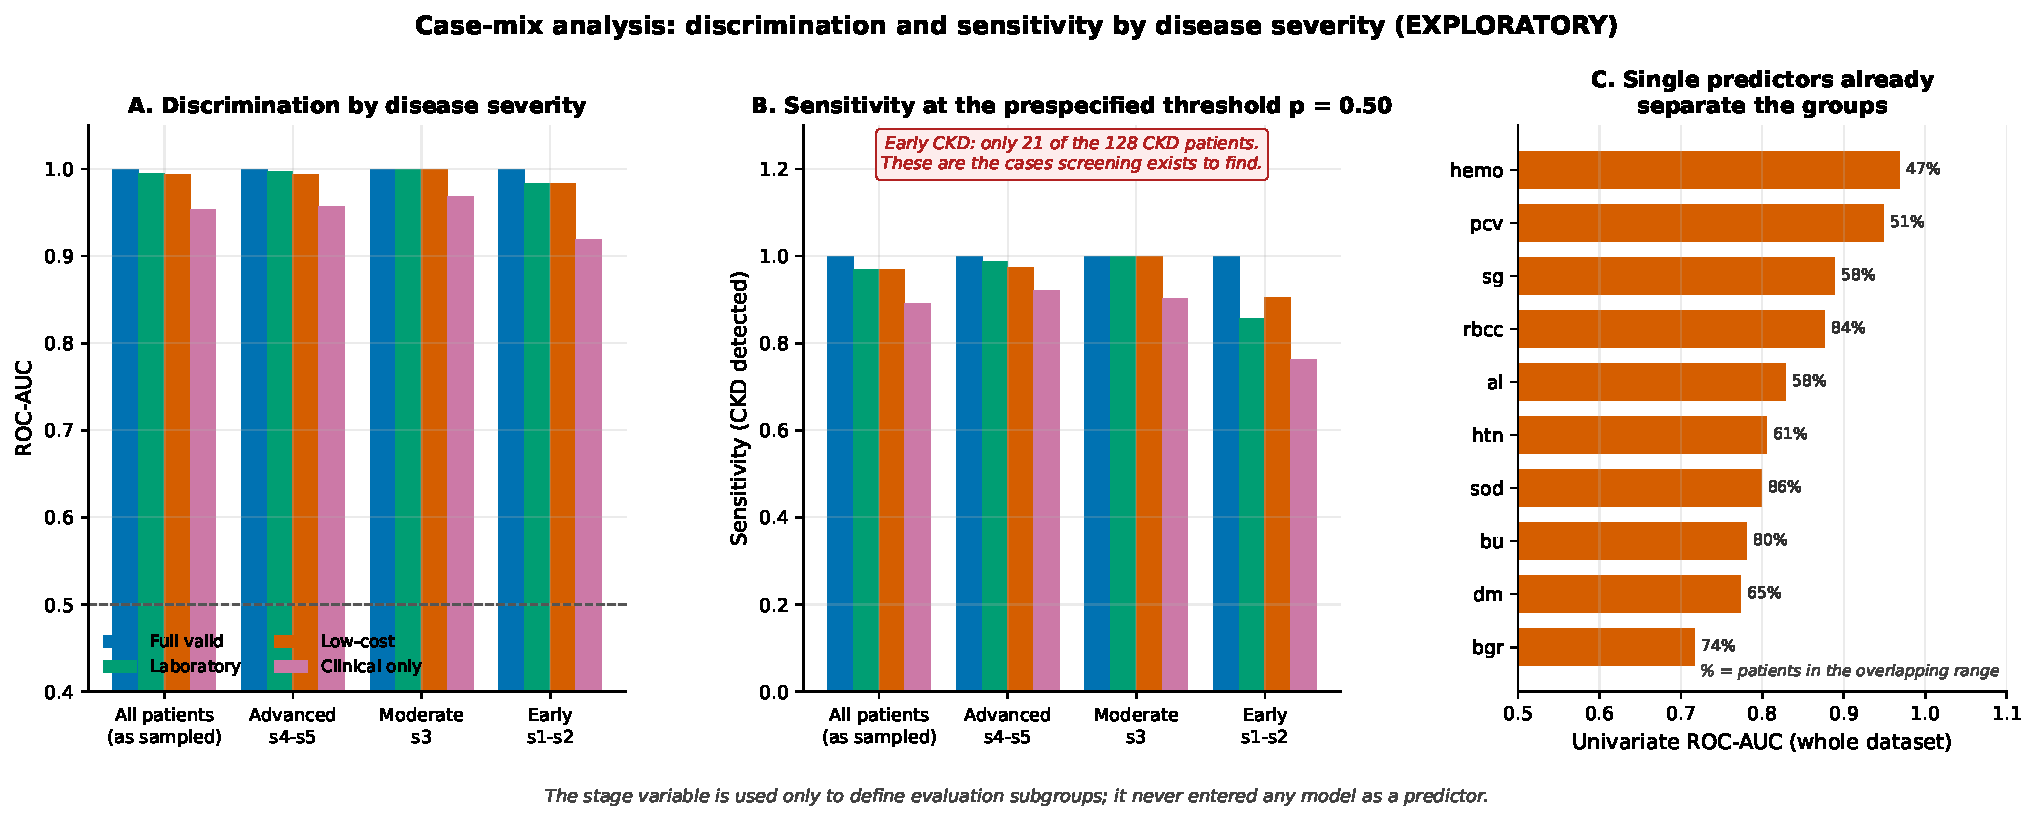
\includegraphics[width=0.92\textwidth]{fig_r12_spectrum_effect.pdf}
\caption{Performance by disease-stage subgroup. Discrimination measured on the
sample as a whole appears optimistic relative to the early-stage patients that
screening exists to find; the early subgroup contains only 21 cases, so these
comparisons are exploratory and hypothesis-generating rather than estimates.
Panel C shows that single predictors already separate the groups, which is why
no multivariable learning is required to reach the ceiling.}
\label{fig:spectrum}
\end{figure*}

\subsection{Mechanism 3: pseudo-external validation}
\label{sec:mech3}

The two mechanisms above concern a single dataset. The third concerns how the
dataset is used. Several published studies train on the 2015 UCI release and
validate on this file---distributed separately, with a different stated
collection site, sample size and year---and present the result as external
validation. That inference requires the two releases to contain different
patients.

They do not. Applying the gate of Section~\ref{sec:gate}
(Fig.~\ref{fig:prov}):

\begin{itemize}
  \item \textbf{All 200} patients match into the 2015 release; the maximum
        bipartite match fraction is \textbf{1.000}.
  \item \textbf{187 of 200} patients are compatible with exactly \emph{one}
        record; the maximum anywhere is two.
  \item Across those 187 uniquely pinned pairs, \textbf{ten categorical
        variables that took no part in the matching agree with zero
        contradictions} ($\approx$1{,}500 comparisons):
        \texttt{rbc}/\texttt{pc} $1\!\leftrightarrow\!$abnormal,
        \texttt{pcc}/\texttt{ba} $1\!\leftrightarrow\!$present,
        \texttt{htn}/\texttt{dm}/\texttt{cad}/\texttt{pe}/\texttt{ane}
        $1\!\leftrightarrow\!$yes, \texttt{appet}
        $1\!\leftrightarrow\!$poor.
\end{itemize}

\textbf{Choosing a null that is hard to beat.} Independent column permutation
destroys every cross-variable relationship, so beating it establishes only
that candidate records are internally coherent; it yields
$0.003 \pm 0.004$. We therefore added a stricter null: within each outcome
stratum we fit a Gaussian copula to the candidate ranks, draw synthetic
records, and map them back through the empirical marginals, producing a
cohort with the right marginal distributions \emph{and} approximately the
right dependence structure but no correspondence to any real patient. That
null yields $\mathbf{0.055 \pm 0.013}$ (maximum 0.105 over 100 draws), which
the observed 1.000 exceeds by roughly 73 standard deviations
(Fig.~\ref{fig:provsens}).

We also record a null that \emph{cannot} be used, because the point is easy
to get wrong: permuting whole candidate rows leaves the statistic exactly
unchanged, since maximum bipartite matching depends only on the multiset of
candidate records and not on their order. We verified this empirically
(1.000 $\rightarrow$ 1.000) and report it as a property of the estimator
rather than as evidence.

\textbf{Sensitivity of the verdict.} Table~\ref{tab:provsens} reports the
matching under varied conditions. Three results matter. Removing the outcome
constraint entirely leaves the match fraction at 1.000 with 182 unique pins,
so the correspondence is carried by the predictors, not by the label.
Dropping each containment variable in turn never reduces the match fraction
below 1.000, though unique pins fall to as few as 133, and removing the five
variables most affected by the release's constant imputation
(Section~\ref{sec:imputation}) still leaves 131 unique pins. Varying the
numeric tolerance from exact containment to $10^{-2}$ changes unique pins
only from 187 to 179.

A fourth result is a caution about the statistic rather than the verdict.
Matching on a four-variable subset also returns a match fraction of 1.000 ---
but with \emph{zero} unique pins and up to 19 candidate partners per patient.
Match fraction saturates once enough candidates are compatible with each
record, so it is not sufficient evidence on its own. \emph{Uniqueness} is
what carries the argument here, and it is uniqueness that the copula null and
the held-out categorical agreement corroborate.

\begin{figure}[t]
\centering
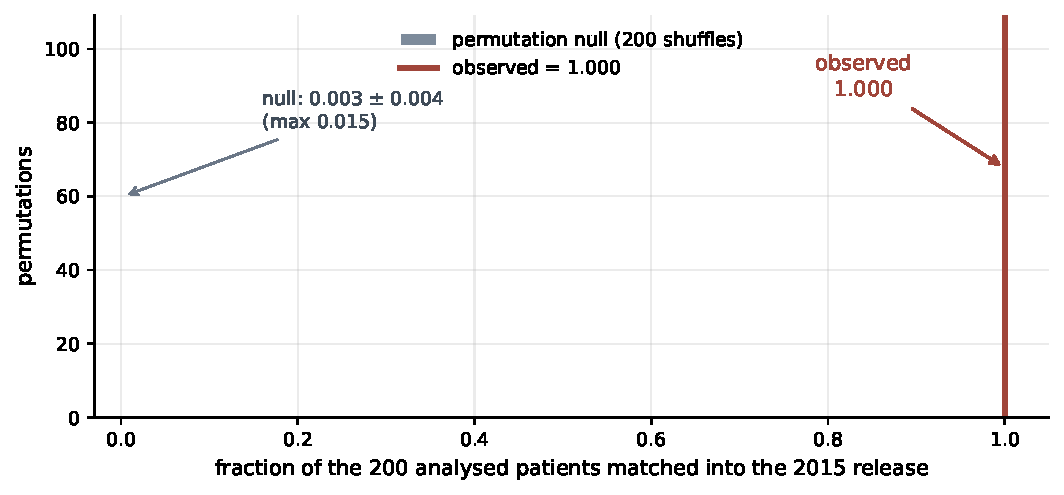
\includegraphics[width=\columnwidth]{fig_r15_provenance_null.pdf}
\caption{Cohort-overlap evidence. The observed match fraction (1.000) against
a permutation null that preserves every marginal distribution while destroying
cross-variable structure. A coincidental alignment does not reproduce ten
variables that played no part in the matching.}
\label{fig:prov}
\end{figure}

% Source: reports/tables/table_44_provenance_sensitivity.csv
\begin{table}[t]
\caption{Sensitivity of the record-level match. Match fraction saturates once
several candidates are compatible with each record; \emph{unique pins} is the
discriminating statistic.}
\label{tab:provsens}
\centering
\footnotesize
\setlength{\tabcolsep}{3pt}
\begin{tabular}{lccc}
\toprule
\tabhead{Condition} & \tabhead{$k$} & \tabhead{Match} &
\tabhead{Unique pins} \\
\midrule
Primary (outcome used)              & 13 & 1.000 & 187 \\
Outcome excluded                    & 13 & 1.000 & 182 \\
Imputation-affected removed         &  8 & 1.000 & 131 \\
Leave-one-variable-out (range)      & 12 & 1.000 & 133--187 \\
Tolerance $0$ to $10^{-2}$          & 13 & 1.000 & 179--187 \\
Laboratory subset                   &  9 & 1.000 & 42 \\
Cheap subset (saturated)            &  4 & 1.000 & 0 \\
\midrule
Negative control (synthetic)        & 13 & 0.005 & 1 \\
\bottomrule
\end{tabular}
\end{table}

\begin{figure}[t]
\centering
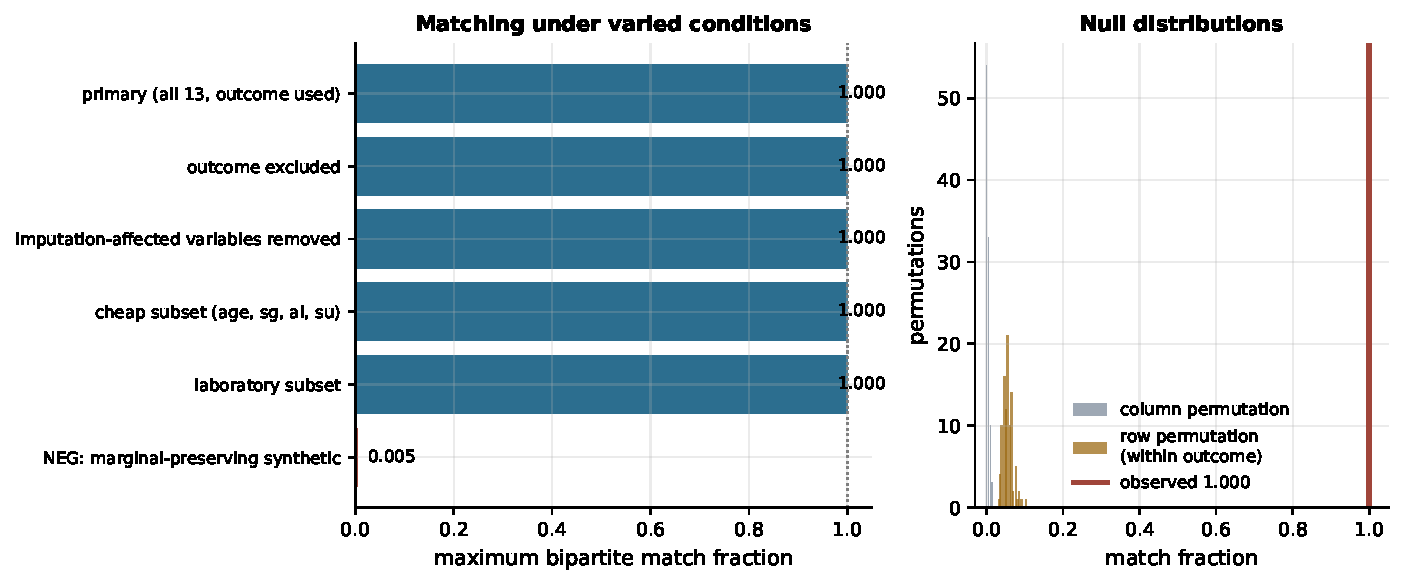
\includegraphics[width=\columnwidth]{fig_provenance_sensitivity.pdf}
\caption{Left: match fraction under varied matching conditions, with the
synthetic negative control in red. Right: the observed match against two
nulls --- independent column permutation, and the stricter copula null that
preserves marginals and correlations.}
\label{fig:provsens}
\end{figure}

A coincidental alignment does not reproduce ten unused variables, survive the
removal of any single variable, or arise in a cohort matched on marginals and
correlations. We state the conclusion at the strength the evidence supports:
\textbf{the data provide strong record-level evidence that the 2020 release is
a discretised subset or re-release of patients represented in the 2015
release}. We do not claim exact raw-value identity, which the discretisation
makes untestable, and we have not contacted the repository maintainers, so
nothing here is an officially confirmed provenance correction.

Of the 13 studies examined in Section~\ref{sec:priorwork}, three validate
across the two releases as though they were independent cohorts, and one
merges them into a single training set before reporting accuracy. On this
evidence those procedures evaluate models on their own training population.

This is not a criticism of those authors. Nothing in either dataset's
documentation indicates the overlap, and the present study registered the 2015
release as its \emph{own} primary external-validation candidate before the
gate refused it.

\subsection{What the discretisation destroyed}

Because the overlap is with a continuous-valued release of the \emph{same
patients}, the cost of the published binning is measurable within-cohort: no
population shift, no case-mix difference, no sampling variation. Recovery is
restricted to the 187 uniquely pinned patients, and every recovered value is
verified to lie inside its own patient's published interval.

% Source: reports/tables/table_31_binning_cost.csv
\begin{table}[t]
\caption{Univariate separability, binned versus recovered continuous values,
evaluated on the same patients. Selected variables.}
\label{tab:binning}
\centering
\small
\begin{tabular}{lccc}
\toprule
\tabhead{Variable} & \tabhead{Binned} & \tabhead{Continuous} &
\tabhead{Lost to binning} \\
\midrule
\texttt{sc}   & 0.680 & 0.946 & $+0.266$ \\
\texttt{pot}  & 0.518 & 0.588 & $+0.070$ \\
\texttt{sod}  & 0.806 & 0.820 & $+0.014$ \\
\texttt{hemo} & 0.985 & 0.985 & $-0.000$ \\
\texttt{sg}   & 0.913 & 0.913 & $\phantom{-}0.000$ \\
\bottomrule
\end{tabular}
\end{table}

The loss is concentrated in one variable, and it is the diagnostically
decisive one (Table~\ref{tab:binning}, Fig.~\ref{fig:binning}). Serum
creatinine loses \textbf{0.266} ROC-AUC; every other variable loses at most
0.070. The published bins explain why: the interval \texttt{< 3.65} absorbs
137 of 177 patients and spans 0.5--3.6~mg/dL---from unambiguously normal
(0.6--1.2) through severe renal impairment---and is only 52\% CKD, while every
other bin is 100\% CKD. In this release serum creatinine is not a graded
measurement but a coarse flag that fires only once creatinine is already
extreme.

\begin{figure}[t]
\centering
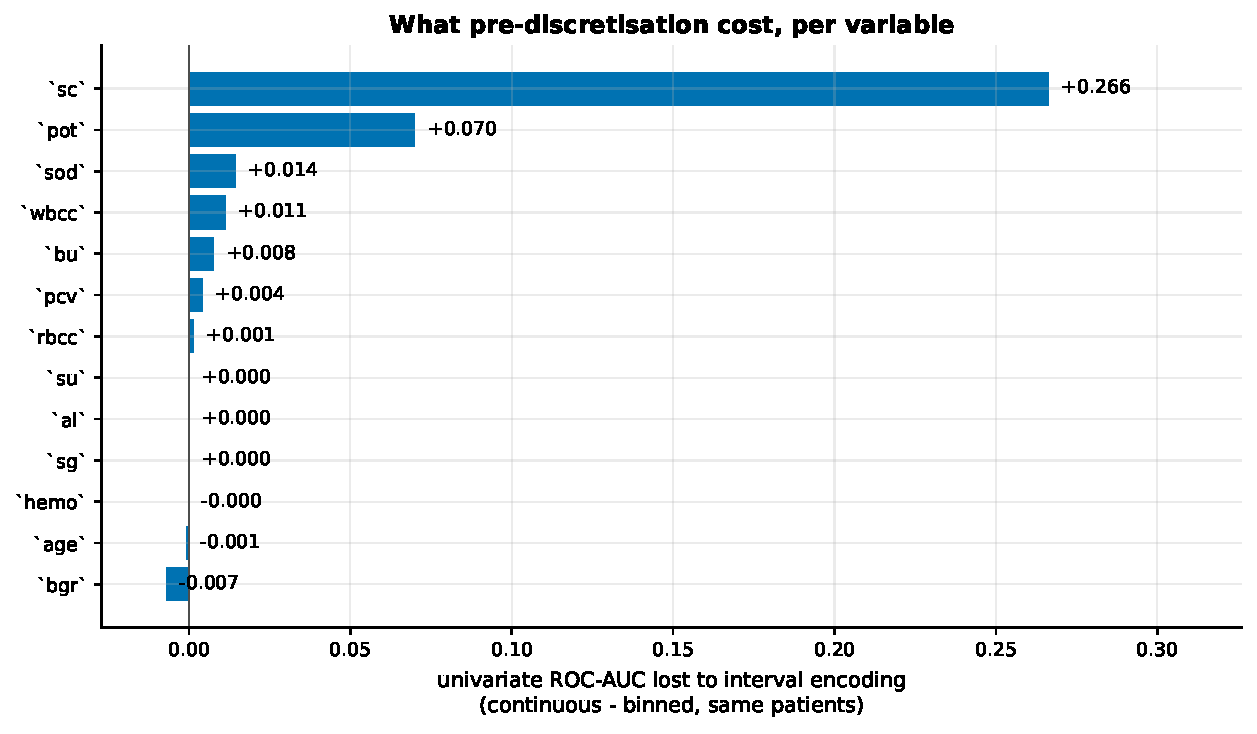
\includegraphics[width=\columnwidth]{fig_r14_binning_cost.pdf}
\caption{Univariate ROC-AUC lost to the published interval encoding, per
variable, on the same patients. The loss is negligible everywhere except serum
creatinine.}
\label{fig:binning}
\end{figure}

This has a consequence for where the leakage boundary should be drawn. We
excluded \texttt{grf} as a post-diagnosis derivative but retained serum
creatinine, on the grounds that it is a routinely measured analyte rather than
a diagnostic label. On the released data that judgement is comfortable
\emph{because binning has flattened the variable}. On the underlying
measurements it is much less so: creatinine alone reaches 0.946, close to the
quantity that defines the outcome. A study using the continuous release would
need to defend that inclusion far more carefully---and could not learn this
from the released file alone.

\subsection{Undocumented constant imputation}
\label{sec:imputation}

The recovery surfaced a second property of the release. The analysed file
contains exactly one missing cell; its source contains many. Across the
recoverable variables, \textbf{339} cells that the source leaves blank carry
values here, and for \textbf{all 13} variables every such cell was filled with
a \emph{single constant}---in each case the clinically normal range
(\texttt{sod} $\rightarrow$ \texttt{133 - 138}, \texttt{rbcc} $\rightarrow$
\texttt{4.46 - 5.05}, \texttt{al} $\rightarrow$ zero).

The missingness is not random. A patient with CKD is 4.9 to over 30 times more
likely to have these measurements absent from the source, which is what one
expects when tests are ordered selectively. Filling every such cell with the
normal value therefore assigns normal-looking laboratory results to precisely
the patients most likely to be ill, and does so invisibly: nothing in the
released file distinguishes a measured normal result from a supplied one.

We state its direction plainly because it runs \emph{against} this paper's
thesis. Every other mechanism examined here inflates measured performance;
this one deflates it, since substituting normal values for the sickest
patients makes the classes harder to separate. The implication is not that the
benchmark is harder than it looks---it is that a substantial minority of some
columns are not measurements at all, which no analysis of the released file
could discover.

\subsection{Would the continuous data have changed any conclusion?}

We modelled the same 187 patients twice under identical design, seeds and
pipelines, differing only in the representation of the recoverable variables.
The largest difference in either direction is \textbf{0.0122} ROC-AUC---an
order of magnitude inside the intervals of Section~\ref{sec:honest}. Nothing
changes.

That null is more informative than a difference would have been. Serum
creatinine gains 0.266 ROC-AUC on its own when its true values are restored,
and the multivariable models do not benefit at all, because the ceiling means
that information is already present several times over via haemoglobin and
packed cell volume. \emph{One can destroy the resolution of the most
diagnostic laboratory analyte in the dataset and the models will not notice.}
What this rules out is the specific worry that the published binning explains
the benchmark's ceiling. It does not; the case mix does.

\subsection{Honest uncertainty}
\label{sec:honest}

Conventional intervals resample patients over pooled out-of-fold predictions
while holding the \emph{fitted models} fixed, and therefore cannot see the
variability introduced by model selection, tuning and calibration being
re-made on a different sample. We removed that shortcut: for each resample the
entire nested procedure is re-run from scratch, 200 times per cell.

Within each resample the outer folds are formed over \emph{patients} rather
than rows, so every copy of a duplicated patient stays on the same side of
every split. Without that constraint a model would be evaluated on patients it
had trained on---the failure this paper is about, and not excusable in its own
methods.

% Source: reports/tables/table_38_procedure_bootstrap.csv
\begin{table}[t]
\caption{Prediction-level versus whole-procedure 95\% intervals for ROC-AUC.
200 resamples per cell, no failures.}
\label{tab:boot}
\centering
\footnotesize
\setlength{\tabcolsep}{3pt}
\begin{tabular}{llccc}
\toprule
\tabhead{Config.} & \tabhead{Model} & \tabhead{Pred.-level} &
\tabhead{Proc.-level} & \tabhead{Ratio} \\
\midrule
Laboratory & SVM & 0.988--0.999 & 0.970--0.999 & 2.7$\times$ \\
Low-cost   & RF  & 0.981--0.999 & 0.968--0.999 & 1.7$\times$ \\
Low-cost   & SVM & 0.979--0.999 & 0.960--0.998 & 1.8$\times$ \\
Full valid & SVM & degenerate   & 0.999--1.000 & --- \\
\bottomrule
\end{tabular}
\end{table}

The honest intervals are 1.7--2.7$\times$ wider (Table~\ref{tab:boot}). These
are the intervals a reader should use when asking whether two configurations
differ; on this evidence, the study's inability to distinguish the low-cost
and laboratory sets is if anything \emph{understated} by the narrower
intervals conventionally reported.

\subsection{Robustness}

Table~\ref{tab:robust} summarises analyses that test whether the conclusions
depend on specific choices. None does.

\begin{table}[t]
\caption{Robustness analyses}
\label{tab:robust}
\centering
\small
\begin{tabular}{p{4.4cm}p{3.1cm}}
\toprule
\tabhead{Question} & \tabhead{Answer} \\
\midrule
Do the 4 internally contradictory labels drive results? &
Deleting: no ($|\Delta| \leq 0.0025$). \textbf{Flipping}: costs low-cost up to
\textbf{0.0241} vs 0.0022 for laboratory. \\
Is the midpoint encoding load-bearing? &
No. Four encodings incl.\ one-hot (86 columns); largest deviation
\textbf{0.0101}. \\
How much is internal validation already correcting for? &
Largest apparent-minus-nested optimism \textbf{+0.0072}. \\
Does isotonic really beat Platt at $n=200$? &
Yes. \textbf{105/120} paired wins (88\%) at 100 outer test sets. \\
\bottomrule
\end{tabular}
\end{table}

The label-robustness asymmetry deserves note because it stresses the paper's
own supporting claim: the four disputed patients are precisely those whose
history, examination and dipstick findings look unremarkable while their
laboratory values indicate advanced disease. If their \texttt{notckd} labels
are the errors, they are exactly the patients a low-cost instrument would
miss---and a laboratory panel would not.

The calibration result is worth one further line, since it contradicts the
usual small-sample expectation. Across 100 outer test sets, isotonic
calibration achieved median Brier 0.0288 against 0.0337 for Platt scaling and
0.0345 uncalibrated, with median calibration slope 1.148 against 2.378 and
1.887 respectively.

\subsection{Supporting result: cost-stratified feature sets}

Under leakage-controlled validation, 11 variables obtainable from history,
examination and a urine dipstick reach ROC-AUC 0.992 (95\% CI 0.981--0.999)
against 0.995 for the 14-variable laboratory panel---a difference well inside
either interval, and unresolved at this sample size.

At identical cost, the additive EBM gives up only 0.0066 ROC-AUC to the RBF
SVM (0.987 vs 0.993) while achieving a calibration slope of \textbf{1.009}
against \textbf{1.257}, and yields per-variable shape functions a clinician
can read and challenge (Fig.~\ref{fig:ebm}). On this sample the readable model
is also the better-calibrated one, so the usual
accuracy-versus-interpretability trade-off does not bind. One caveat is
recorded rather than smoothed over: \texttt{bp (Diastolic)} runs opposite to
its own marginal association---a suppression effect beside \texttt{bp limit}
and \texttt{htn}---and must not be read in isolation.

\begin{figure*}[t]
\centering
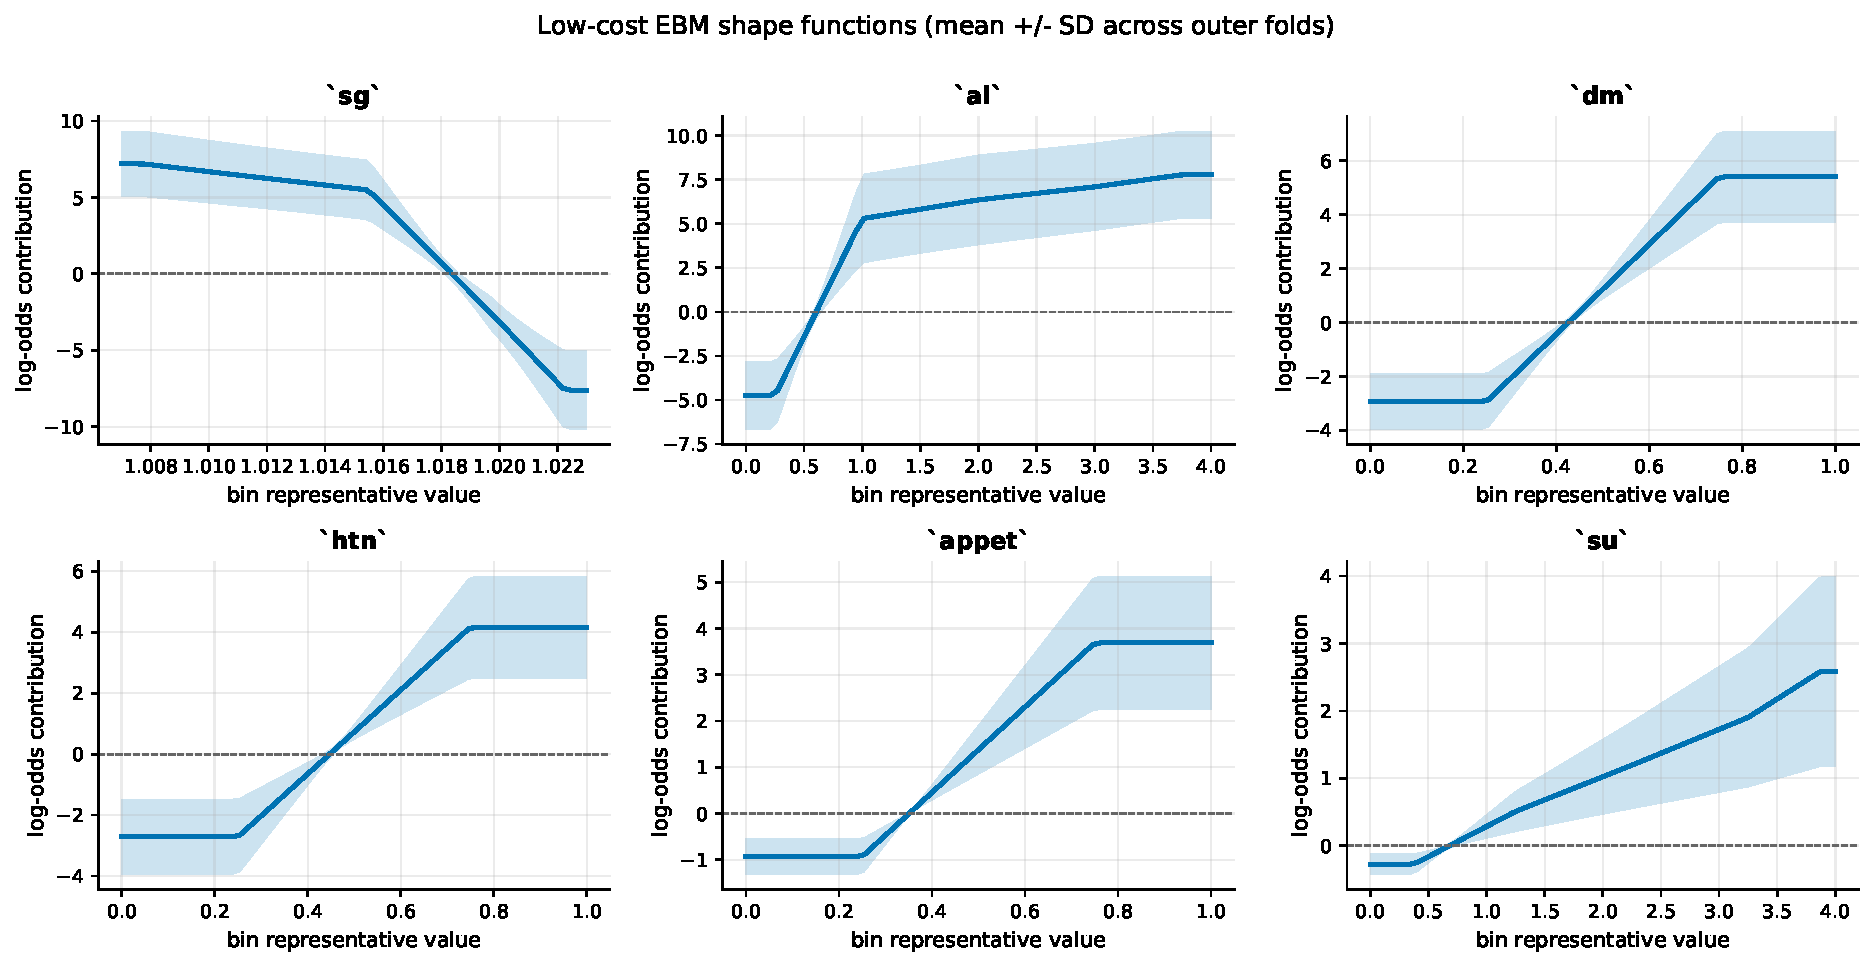
\includegraphics[width=0.92\textwidth]{fig_r13_ebm_shapes.pdf}
\caption{Fitted shape functions of the low-cost additive model, averaged over
25 outer folds (shaded band: $\pm 1$ SD). Directions are clinically coherent:
low urine specific gravity raises risk, albuminuria raises it steeply, and
diabetes, hypertension and poor appetite all push the same way.}
\label{fig:ebm}
\end{figure*}

\textbf{This is a statement about cost tiers on this case mix. It is not a
screening result}, because a sample in which 84\% of cases carry
moderate-to-severe disease is not a screening population.

\subsection{A transportability probe on an independent cohort}
\label{sec:external}

Every result above is internal. The provenance gate disqualified the obvious
external candidate (Section~\ref{sec:mech3}), leaving one registered source
that carries the \emph{same measurements} on different patients: the MIMIC-IV
critical-care demonstration database, from a different country and health
system. We extracted 100 subjects in this study's schema---26 coded CKD by
ICD-10 \texttt{N18*} or ICD-9 \texttt{585*}, with nine blood analytes at
92--94\% coverage plus urine specific gravity.

We describe this experiment as a \emph{transportability probe} or stress
test, not as an external validation of the kind that would support a
performance claim. A validation cohort would need to be adequately powered,
drawn from a population in which the model is intended to operate, and
labelled by the same standard as the development data. This cohort satisfies
none of those conditions: it contributes 20 cases, comes from critical care,
and is labelled administratively. What it can do---and what a validation
cohort is not needed for---is test whether performance near the ceiling
persists when the patients change at all.

Three properties of the extraction are load-bearing. The derived label is
named so that the registry's prohibited-column declaration, written before
the extraction existed, already covers it. A \emph{temporal guard} discards
laboratory values that do not strictly precede the admission at which CKD was
first coded, removing 8{,}754 values. And the six subjects left with no
eligible measurement are reported rather than imputed into existence.

Models were trained on all 200 analysed patients and applied \textbf{without
any refitting}. The transfer feature set is the intersection of the two
schemas---ten variables---passed as a ``feature override'' on the existing
valid configuration so that both leakage guards still run. An internal
reference is computed on exactly that feature set, so the drop caused by
transfer is separable from any drop caused by using fewer variables.

% Source: reports/tables/table_42_external_validation.csv
\begin{table}[t]
\caption{Frozen transfer to an independent cohort. Internal reference and
external result use the same ten variables.}
\label{tab:external}
\centering
\footnotesize
\setlength{\tabcolsep}{3pt}
\begin{tabular}{lccccc}
\toprule
\tabhead{Model} & \tabhead{Int.\ AUC} & \tabhead{Ext.\ AUC (95\% CI)} &
\tabhead{Brier} & \tabhead{Sens.} & \tabhead{Spec.} \\
\midrule
Logistic  & 0.997 & 0.702 (0.594--0.794) & 0.409 & 0.95 & 0.47 \\
SVM       & 0.997 & 0.699 (0.599--0.788) & 0.423 & 0.95 & 0.45 \\
Random forest & 0.997 & 0.708 (0.605--0.803) & 0.418 & 0.95 & 0.39 \\
\bottomrule
\end{tabular}
\end{table}

\textbf{Discrimination falls sharply on the new cohort.} Internal ROC-AUC on
this feature set is 0.997; on the probe cohort it is 0.699--0.708, a fall of
roughly 0.29 (Table~\ref{tab:external}). All three model families agree, and
the bootstrap intervals exclude the internal estimate by a wide margin. The
inference this supports is a conditional one: performance measured near the
ceiling on this benchmark is not, on this evidence, a reliable guide to
performance on a different patient population. It does not by itself
establish how much of the internal figure was optimism, and we quantify
neither.

\textbf{Calibration fails worse, and for a legible reason.} External Brier
scores are 0.409--0.423 against 0.014 internally, with calibration intercepts
far below zero: the models assign high risk to almost everyone. At the
prespecified threshold they retain sensitivity 0.95 while specificity
collapses to 0.39--0.47. Prevalence is the obvious culprit---64\% in training
against 21\% externally. Applying recalibration-in-the-large, the minimal
correction a deployer would make, reduces the Brier score to 0.172--0.175. It
cannot change the ranking, so discrimination is unmoved by construction, and
it leaves no prediction above 0.50, so the model flags nobody at the
prespecified threshold. \emph{The binding constraint is the discrimination of
0.70, not the calibration}, and no post-hoc correction addresses it.

\textbf{The difference cannot be attributed to internal optimism alone.}
This design cannot decompose it, and at least six mechanisms plausibly
contribute:

\begin{itemize}
  \item \emph{Small-sample uncertainty.} The probe rests on 20 cases and 74
        controls; the interval spans 0.59--0.80, so the point estimate is
        itself imprecise.
  \item \emph{Case-mix differences.} The development sample is 84\% stage
        3--5 with 64\% prevalence; the probe cohort is critical-care with
        21\% prevalence and a different severity profile.
  \item \emph{Measurement and feature definition.} Analytes are drawn from
        hospital laboratory systems under different assay and reporting
        conventions, and the urine dipstick tier is semi-quantitative text
        mapped to an ordinal scale rather than natively recorded.
  \item \emph{Missingness differences.} The development file contains one
        missing cell because the release imputed the rest with constants
        (Section~\ref{sec:imputation}); the probe cohort has genuine
        missingness imputed within training folds. The two arms therefore
        differ in how absent measurements are represented.
  \item \emph{Clinical setting.} Critical-care admission selects patients on
        acute physiology, which perturbs precisely the analytes the models
        rely on.
  \item \emph{Genuine population and distribution shift}, including
        differences in country, health system, era and coding practice.
\end{itemize}

Internal optimism is a seventh candidate, and the study offers indirect
support for it---the honest intervals of Section~\ref{sec:honest} and the
saturation behaviour of Section~\ref{sec:bid} both indicate a sample that
should not be expected to transfer---but the probe does not isolate it.
Attributing the fall to any single mechanism, optimism included, would
overstate what a 20-case comparison can support.

None of this diminishes what the probe contributes. It is the only evidence
in the study drawn from patients the models had never seen, it is the only
such evidence the registered sources permit once the provenance gate has
excluded the alternative, and its direction is unambiguous and consistent
across three model families. A benchmark whose reported discrimination is
0.99 and whose models score 0.70 on the first independent cohort available
warrants the caution this paper argues for, whatever the decomposition of
that gap turns out to be.

%==============================================================================
\section{A Proposed Diagnostic for Benchmark Informativeness}
\label{sec:bid}

Every mechanism above was invisible in the number the literature reports.
That is not an accident of this dataset. Discrimination answers ``how well
did this model separate these patients?'' and says nothing about whether the
dataset can distinguish good methods from bad ones. This section proposes
three measurements that address the gap and applies them here.

We state the provenance of the idea plainly: none of the three components is
new. Direct standardisation is routine in epidemiology, learning curves are
long established, and comparing a model against a strong single-feature
baseline is ordinary practice. What is proposed is their composition into a
\emph{benchmark-level} check that can be run before a dataset is trusted,
with reporting thresholds. Those thresholds are calibrated on one benchmark
and are offered for discussion, not as standards.

\subsection{Multivariable lift}

How much did modelling add over the single most separable column? We report
$\mathrm{AUC}(\text{model}) - \mathrm{AUC}(\text{best single predictor})$,
with a paired patient-level bootstrap interval. The baseline is given the
benefit of the doubt: a single raw column has no fitted direction, so its AUC
is taken as $\max(\mathrm{AUC}, 1-\mathrm{AUC})$, which makes the lift
smaller rather than larger.

% Source: reports/tables/table_43_bid_lift.csv
\begin{table}[t]
\caption{Multivariable lift over the best single predictor.}
\label{tab:lift}
\centering
\footnotesize
\setlength{\tabcolsep}{3.5pt}
\begin{tabular}{lccc}
\toprule
\tabhead{Configuration} & \tabhead{Model} & \tabhead{Best single} &
\tabhead{Lift (95\% CI)} \\
\midrule
Low-cost (11)   & 0.993 & \texttt{sg} 0.888   & $+0.105$ (0.071, 0.145) \\
Laboratory (14) & 0.994 & \texttt{hemo} 0.968 & $+0.026$ (0.010, 0.043) \\
Full valid (25) & 1.000 & \texttt{hemo} 0.968 & $+0.032$ (0.014, 0.053) \\
\bottomrule
\end{tabular}
\end{table}

The laboratory configuration---fourteen variables, a full blood panel and
urine microscopy---improves on haemoglobin \emph{alone} by 0.026 ROC-AUC
(Table~\ref{tab:lift}). The full valid configuration, with 25 variables, adds
0.032. A benchmark on which the entire modelling exercise is worth three
hundredths of an AUC over one raw measurement cannot rank methods, whatever
numbers it produces. The low-cost set is the informative exception at
$+0.105$: it is the one place in this study where combining variables
demonstrably works, which is consistent with its variables being
non-redundant rather than proxies for one another.

\subsection{Saturation}

How much of the training data was needed? Using 10\% of each training
fold---roughly 16 patients---already reaches ROC-AUC 0.970, against 0.996 on
the full fold. Ninety per cent of the achievable gain above chance arrives at
10\% of the data (Fig.~\ref{fig:saturation}). A benchmark solved by a tenth
of its training examples cannot reward sample efficiency, and its reported
numbers describe the task rather than the learner.

\begin{figure}[t]
\centering
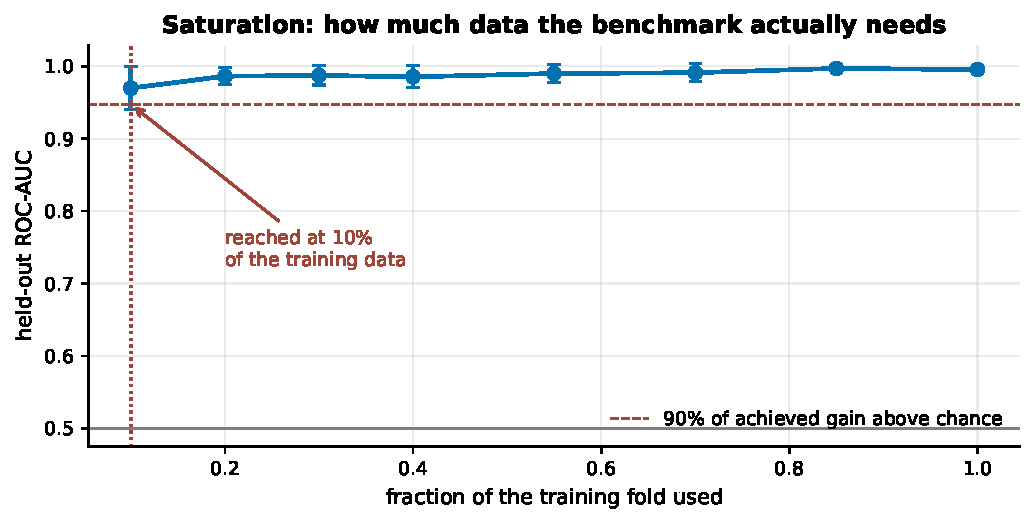
\includegraphics[width=\columnwidth]{fig_r16_bid_saturation.pdf}
\caption{Held-out discrimination against the fraction of the training fold
used. The curve is flat from a tenth of the data onward, so the benchmark
cannot distinguish methods by how efficiently they learn.}
\label{fig:saturation}
\end{figure}

\subsection{Case-mix standardisation, and a negative result}

What would the numbers be in a population with a stated severity mix? We
re-weight cases to the case mix of a published community screening
series~\cite{kabir2026} (22\% stage 1, 46\% stage 2, 32\% stage 3) and
recompute. Standardising the \emph{AUC} moves it by at most 0.008---so on
this evidence it would not flag a benchmark that Section~\ref{sec:mech2} shows is
case-mix dependent at a threshold.

The explanation is specific to this dataset, and stating it precisely
matters. AUC is a rank statistic, so re-weighting which cases are present
moves it only insofar as it changes whether cases outrank controls. Here even
the early-stage cases are well separated---their subgroup ROC-AUC is 0.983,
on 21 cases and therefore imprecise---so shifting weight toward them changes
few rankings. Sensitivity at a fixed threshold has no such invariance: a case
below the threshold is missed however it ranks, and the same re-weighting
shifts it by up to 0.056, an order of magnitude more, flagging the laboratory
configuration. Because the re-weighting concentrates on a 21-case stratum,
the standardised quantities inherit that imprecision and are reported as
exploratory; the effective case count after weighting is 38.2, and we draw no
inference from the standardised values other than the qualitative contrast
between the two metrics' sensitivity to case mix.

This is \textbf{not} evidence that AUC is generally blind to spectrum
effects. It plainly is not: a case mix that pushes cases below controls does
move AUC, which is why spectrum bias is a recognised threat to discrimination
measures. What this dataset shows is narrower and still useful---a sample can
be separable enough that AUC absorbs a large change in case mix while a
threshold-based metric does not. The practical consequence is that
standardising discrimination alone can give false reassurance, so an
operating-point metric should be standardised alongside it. Which of the two
moves more will depend on the dataset.

Applied here, the protocol raises at least one flag for every configuration,
and reaches that conclusion without reference to any of the three mechanisms
that motivated it. Whether the thresholds transfer is an open question; the
machinery is released so that others can find out.

%==============================================================================
\section{Discussion}

This study set out to measure one failure mode and found three. Each pushes
measured performance toward 1.0, none is predictive ability, and they compound:
controlling any one leaves the others free to produce a near-perfect number.

They are also ordered by how easy each is to miss. Leakage is visible in the
column list. Case mix requires examining who is in the sample. Cohort overlap
requires comparing two datasets nobody had reason to suspect were one---and is
invisible from inside either file, since both look like well-formed,
separately documented datasets. That ordering is the paper's general point: a
benchmark's trustworthiness is not a property one can establish by analysing
it.

Three practices follow, each cheap and each of which changed a conclusion
here. \emph{Declare prohibited columns and enforce them with something that
raises rather than drops.} \emph{Inspect the stage distribution and univariate
separability before believing a discrimination figure}---if a single predictor
reaches 0.97 alone, the modelling is not what is producing the result.
\emph{Verify that a validation cohort is a different set of patients}, by
record-level comparison rather than by documentation.

The transportability probe in Section~\ref{sec:external} lends that argument
empirical support, within limits we state rather than minimise. A model whose
internal discrimination is 0.997 achieves 0.70 on patients it has not seen,
with calibration that would refer almost the entire cohort. The probe is
underpowered at 20 cases, drawn from critical care, and labelled
administratively, so the gap reflects some combination of small-sample
variation, case mix, measurement and feature definition, missingness
handling, clinical setting and distribution shift, alongside any internal
optimism; the design cannot apportion it. The claim it supports is
correspondingly modest and is the one the paper needs: on this benchmark, an
internal figure near 1.0 is a poor guide to performance on different
patients. Establishing \emph{why}, and estimating what performance in an
intended setting would be, requires an adequately powered cohort from that
setting.

The wider implication concerns how benchmark results are read. Two of the
three mechanisms here are properties of the data that no amount of careful
modelling can correct, and the third invalidates the evidence normally taken
as decisive. A reported accuracy of 99\% on this benchmark is compatible with
a model that has learned nothing transferable, and distinguishing the cases
requires exactly the leakage audit, subgroup analysis and provenance check
reported here. Section~\ref{sec:bid} asks the further question of whether the
benchmark can rank methods at all, and answers no: the entire modelling
exercise is worth about 0.03 ROC-AUC over one raw measurement, and a tenth of
the training data suffices.

\subsection{Extension to synthetic tabular and synthetic patient data}
\label{sec:synthetic}

The failure modes documented here are not specific to real data, and the
safeguards generalise directly to pipelines that generate or evaluate
synthetic tabular records. Synthetic-data evaluation is in one respect
harder: a generator trained on a source table can reproduce individual rows,
so the question ``is the evaluation set independent of the training set?''
becomes a question about memorisation as well as provenance, and the
mechanisms of Sections~\ref{sec:mech3} and \ref{sec:gate} answer only the
latter.

Seven components of the protocol we implement are already directly reusable.
Cryptographic dataset fingerprints establish that an input has not silently
changed; here the source file is SHA-256 checksummed on every load and
re-verified in continuous integration. Exact-row and near-duplicate detection
across training, validation, test and reference sets generalises the
interval-containment matching of Section~\ref{sec:mech3}, which is a
tolerance-based near-duplicate test calibrated against a permutation null.
Entity-level overlap checks using stable identifiers, or privacy-preserving
linkage where identifiers cannot be shared, correspond to the bipartite
matching and held-out categorical confirmation reported there.
Feature--target leakage scans and the detection of target proxies and
post-outcome variables correspond to the declared prohibited-column sets and
the outcome-proxy audit of Section~\ref{sec:leakageprev}. Enforcing that all
preprocessing is
fitted inside cross-validation folds is the guard tested here. Provenance
manifests recording origin, version, transformations and split history
correspond to the run manifest and external-dataset registry. And the
fail-closed gate---blocking evaluation when overlap, leakage or undocumented
provenance exceeds a threshold---is implemented as a test that fails when any
non-independent cohort appears in an external-validation table.

Two further components are specific to synthetic data and are \emph{not}
implemented here. Membership-inference and memorisation checks ask whether a
synthetic record discloses that a particular real patient was in the training
set. Nearest-neighbour similarity and distance-to-closest-record diagnostics
ask whether synthetic rows are near-copies of real ones, which is both a
privacy question and an evaluation-validity question: a synthetic test set
whose records sit arbitrarily close to training records reproduces, in a
subtler form, exactly the pseudo-external validation of
Section~\ref{sec:mech3}. Adding them to the gate we release is the natural
next step and we have not taken it; the present work provides the provenance
half of the problem, not the memorisation half.

We note the analogy carries a caution as well as a recipe. The most
consequential mechanism in this study was not leakage but case
mix---something no fingerprint, hash or duplicate scan would detect. A
synthetic cohort can be free of memorisation, pass every overlap check, and
still be uninformative because its severity distribution makes the task
trivial. Diagnostics of the kind proposed in Section~\ref{sec:bid} are
complementary to provenance gating for that reason, and we would expect a
mature synthetic-data evaluation pipeline to run both.

%==============================================================================
\section{Limitations}

Model development rests on 200 patients, and \textbf{the study has no
adequately powered external validation}. What it has is a transportability
probe (Section~\ref{sec:external}) on 94 subjects and 20 cases. The natural
comparator---the larger 2015 release---is disqualified by our own finding,
and the gate enforces that rather than merely stating it. The probe cohort is
drawn from critical care rather than any screening or general population,
sits in a different country and health system, and carries administratively
coded rather than adjudicated labels with no chronicity criterion verified.
It demonstrates that discrimination measured on this benchmark does not
persist on a different population; it \emph{cannot} apportion that difference
among small-sample uncertainty, case mix, measurement and feature definition,
missingness handling, clinical setting, distribution shift and internal
optimism, and it is far too small and too unrepresentative to estimate what
performance in any intended setting would be. No performance claim for any
population should be drawn from it. The most suitable remaining candidate is
a community-based series with 68\% of cases at stages 1--2, access to which
is restricted.

The sampling is hospital-based and single-centre; the 64\% prevalence is a
property of recruitment, and PPV and NPV reported at that prevalence do not
transfer. The case mix is the most consequential limitation and is why no
figure here estimates screening performance.

\textbf{The early-stage subgroup analysis is exploratory and underpowered.}
It rests on 21 cases, was specified post hoc rather than in advance, and is
reported without formal inferential comparison. Its role in the argument is
to illustrate a case-mix imbalance that is established independently by
arithmetic---107 of 128 cases at stages 3--5---and not to estimate
early-stage performance, which 21 cases cannot support. The direction is
consistent across configurations, but the magnitude should be treated as
hypothesis-generating and requires confirmation in a larger, prospectively
defined early-stage cohort. The same caution applies to the standardised
quantities in Section~\ref{sec:bid}, whose weights concentrate on that
stratum.

Four records are internally
contradictory, and while deleting them changes nothing, trusting their staging
instead costs the low-cost configuration up to 0.0241 ROC-AUC---so this
limitation is half-answered, not answered. The data are cross-sectional, so
chronicity, which the definition of CKD requires, cannot be established. Age is
banded and no sex, ethnicity or socioeconomic variable exists, so
\textbf{subgroup and fairness analysis is impossible}---a reason for caution
rather than an excuse for silence.

The literature survey is targeted rather than systematic, and 10 of its 13
rows await hand verification behind paywalls. This matters more than most
limitations here, because the paper's opening claim is a claim about the
literature.

The diagnostic protocol of Section~\ref{sec:bid} is a proposal, not a
validated instrument. Its thresholds are set from the behaviour of a single
benchmark, its components are individually familiar rather than novel, and
one of them---standardised AUC---failed to flag a dataset it should have,
which we report rather than remove. It should be read as a starting point for
discussion.

Reproducibility has an honest limit: identical seeds reproduce identical
predictions within an environment, but across an environment rebuild
agreement is to approximately $10^{-16}$ rather than bit-for-bit, because
floating-point summation order depends on the installed BLAS.

We make no claim about clinical utility, causality, deployment readiness or
generalisability, and none about \emph{how} the provenance discrepancy arose.

%==============================================================================
\section{Conclusion}

Machine-learning results on this benchmark cluster at the discrimination
ceiling. We identify three mechanisms that put them there. Target leakage
takes any configuration to ROC-AUC 1.000. Case mix---84\% of cases at stage
3--5, with haemoglobin alone at 0.968---puts valid models at the ceiling
unaided, and is the larger effect. And the two releases the literature treats
as independent cohorts share their patients record-for-record, so published
cross-dataset validations between them measure resubstitution.

Transferring the models unchanged to an independent cohort, as a
transportability probe rather than a definitive external validation, then
indicates what those mechanisms may cost: discrimination of 0.997 becomes
0.70, and calibration fails badly enough to refer nearly everyone. With 20
cases from a critical-care population, that difference reflects some
combination of small-sample uncertainty, case mix, measurement definition,
missingness, clinical setting and distribution shift as well as any internal
optimism, and the probe cannot separate them. It bounds the direction rather
than the magnitude---but the direction is the point.

What the work supports is a methodological claim in two parts. About this
benchmark: its reported numbers are largely explained by properties of the
data, the largest of which is rarely examined and the least visible of which
invalidates the cross-dataset validations that would otherwise be its
strongest evidence; and what remains did not transfer to the one independent
cohort we could test. About method: all three mechanisms were found by checks
that can be run \emph{before} any model is fitted---declare and enforce prohibited columns, inspect the case mix and
univariate separability, and verify at record level that a validation cohort
is a different set of patients. We add a fourth question worth asking of any
benchmark before trusting it: does modelling beat the best single column, and
does the task need more than a fraction of the data? On this benchmark the
answers are barely and no. Section~\ref{sec:synthetic} sets out how the same
safeguards, and the two memorisation-specific checks we do not implement,
would apply to synthetic tabular and synthetic patient data.

Prospective validation in a genuine screening series would be required before
any clinical interpretation is warranted, and no dataset examined here can
substitute for it.

%==============================================================================
\section*{Reproducibility}

The complete pipeline, including the provenance gate as reusable
dataset-agnostic machinery, is available in the accompanying repository. One
master seed derives every fold and model seed; the raw file is checksummed on
every load and never modified; all out-of-fold predictions---108{,}000 rows,
being repeated evaluations of 200 unique patients across the full grid---are
written to a single table from which every reported number is derived; and 416
automated tests enforce the leakage, determinism and report-consistency
guarantees, including the provenance gate and the external-cohort temporal
guard. Environment and BLAS build are recorded in a lock file. Reporting
follows the spirit of TRIPOD+AI~\cite{tripod2024}; a completed checklist
accompanies the repository.

%==============================================================================
\begin{thebibliography}{99}

\bibitem{gbd2020}
GBD Chronic Kidney Disease Collaborators,
``Global, regional, and national burden of chronic kidney disease, 1990--2017:
a systematic analysis for the Global Burden of Disease Study 2017,''
\emph{The Lancet}, vol.~395, no.~10225, pp.~709--733, 2020.
doi:10.1016/S0140-6736(20)30045-3

\bibitem{kdigo2024}
Kidney Disease: Improving Global Outcomes (KDIGO) CKD Work Group,
``KDIGO 2024 clinical practice guideline for the evaluation and management of
chronic kidney disease,''
\emph{Kidney International}, vol.~105, no.~4S, pp.~S117--S314, 2024.
doi:10.1016/j.kint.2023.10.018

\bibitem{tripod2024}
G.~S. Collins, K.~G.~M. Moons, P.~Dhiman, \emph{et al.},
``TRIPOD+AI statement: updated guidance for reporting clinical prediction
models that use regression or machine learning methods,''
\emph{BMJ}, vol.~385, e078378, 2024.
doi:10.1136/bmj-2023-078378

\bibitem{uci2015}
L.~Rubini, P.~Soundarapandian, and P.~Eswaran,
``Chronic Kidney Disease,'' UCI Machine Learning Repository, 2015.
doi:10.24432/C5G020

\bibitem{uci2023}
M.~A. Islam and S.~Akter,
``Risk Factor Prediction of Chronic Kidney Disease,''
UCI Machine Learning Repository, 2020.
doi:10.24432/C5WP64

\bibitem{riley2019}
R.~D. Riley, K.~I.~E. Snell, J.~Ensor, \emph{et al.},
``Minimum sample size for developing a multivariable prediction model:
Part II --- binary and time-to-event outcomes,''
\emph{Statistics in Medicine}, vol.~38, no.~7, pp.~1276--1296, 2019.
doi:10.1002/sim.7992

\bibitem{varma2006}
S.~Varma and R.~Simon,
``Bias in error estimation when using cross-validation for model selection,''
\emph{BMC Bioinformatics}, vol.~7, art.~91, 2006.
doi:10.1186/1471-2105-7-91

\bibitem{vancalster2016}
B.~Van Calster, D.~Nieboer, Y.~Vergouwe, B.~De Cock, M.~J. Pencina, and
E.~W. Steyerberg,
``A calibration hierarchy for risk models was defined: from utopia to
empirical data,''
\emph{Journal of Clinical Epidemiology}, vol.~74, pp.~167--176, 2016.
doi:10.1016/j.jclinepi.2015.12.005

\bibitem{nori2019}
H.~Nori, S.~Jenkins, P.~Koch, and R.~Caruana,
``InterpretML: a unified framework for machine learning interpretability,''
arXiv:1909.09223, 2019.

\bibitem{kabir2026}
M.~A. Kabir, S.~Munira, D.~T. Azad, S.~M. Ikram, M.~H.~R. Sarker, and
S.~M.~A. Hanifi,
``Community-based early-stage chronic kidney disease screening using
explainable machine learning for low-resource settings,''
\emph{International Journal of Medical Informatics}, 2026.
arXiv:2601.01119

\bibitem{islam2023}
M.~A. Islam, M.~Z.~H. Majumder, and M.~A. Hussein,
``Chronic kidney disease prediction based on machine learning algorithms,''
\emph{Journal of Pathology Informatics}, vol.~14, art.~100189, 2023.
doi:10.1016/j.jpi.2023.100189

\bibitem{hossain2025}
M.~F. Hossain, S.~T. Diya, and R.~Khan,
``ACD-ML: Advanced CKD detection using machine learning: a tri-phase ensemble
and multi-layered stacking and blending approach,''
\emph{Computer Methods and Programs in Biomedicine Update}, vol.~7,
art.~100173, 2025.
doi:10.1016/j.cmpbup.2024.100173

\end{thebibliography}

\end{document}
